\section{Figuras}

\begin{figure}[h!]
\centering
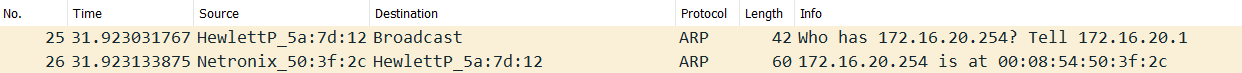
\includegraphics[scale=0.45]{imagens/exp1_ARP.png}
\caption{Pacotes ARP}
\label{fig:arp_packets}
\end{figure}

\begin{figure}[h!]
\centering
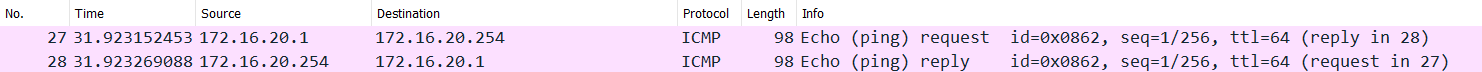
\includegraphics[scale=0.4]{imagens/exp1_ping.png}
\caption{Comando Ping em pacotes ICMP}
\label{fig:icmp_packets}
\end{figure}

\begin{figure}[h!]
\centering
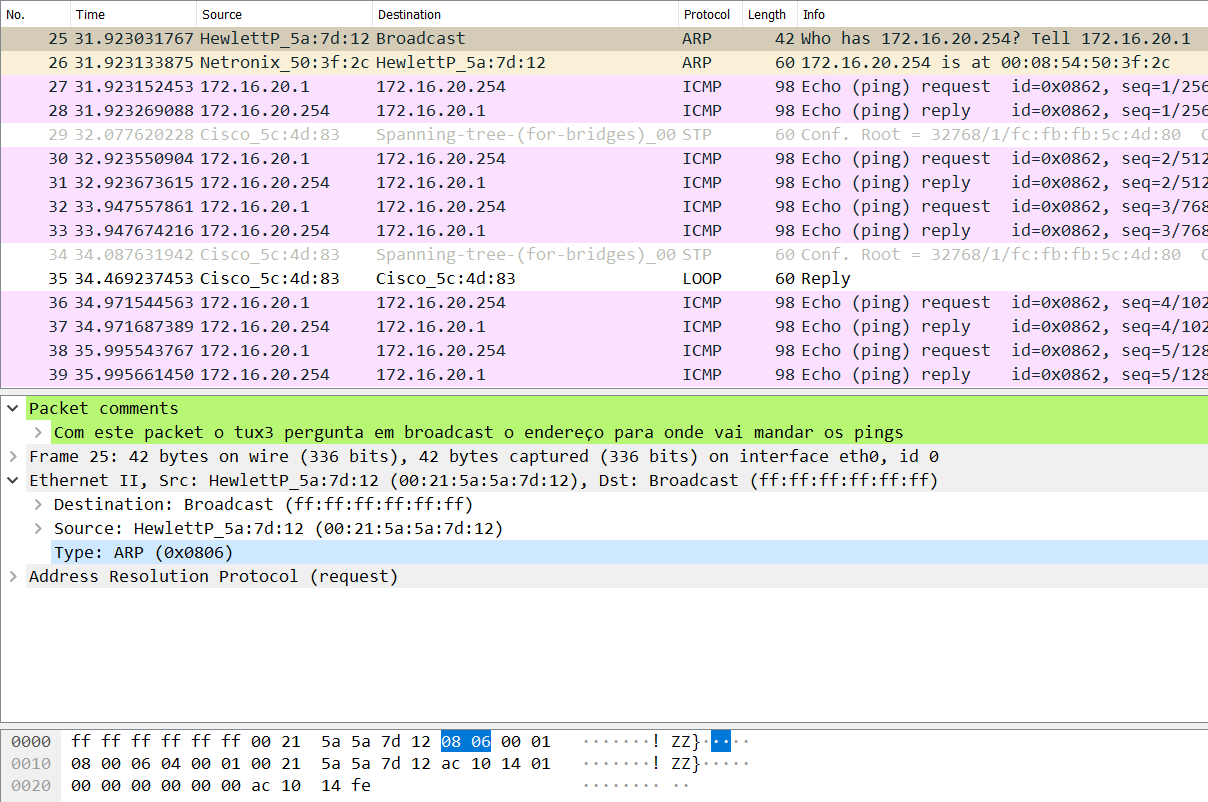
\includegraphics[scale=0.4]{imagens/exp1_type_arp.png}
\caption{Determinação de pacotes do tipo ARP via wireshark}
\label{fig:arp_wireshark}
\end{figure}

\begin{figure}[h!]
\centering
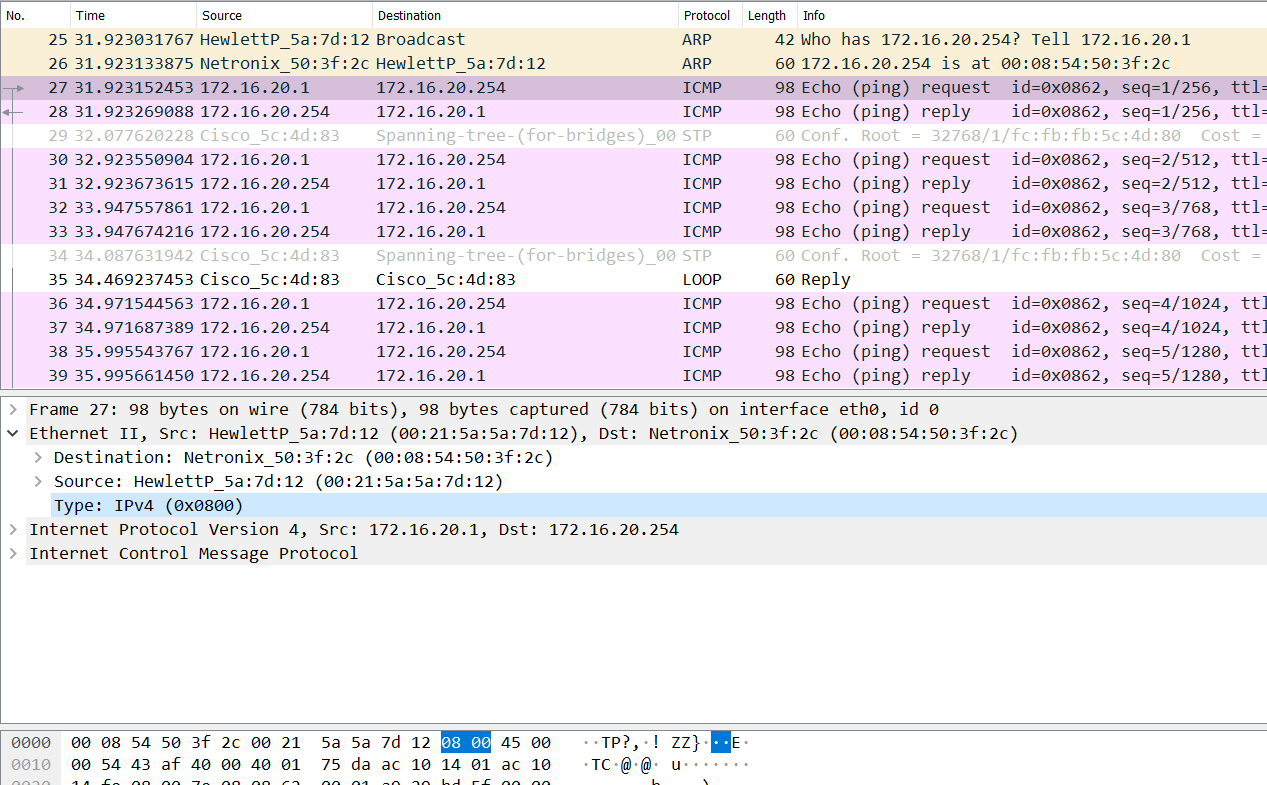
\includegraphics[scale=0.4]{imagens/exp1_type_icmp.png}
\caption{Determinação de pacotes do tipo ICMP via wireshark}
\label{fig:icmp_wireshark}
\end{figure}

\begin{figure}[h!]
\centering
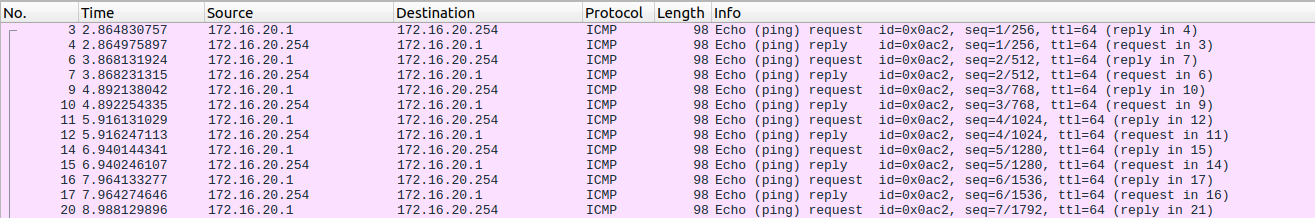
\includegraphics[width=\textwidth,height=\textheight,keepaspectratio]{imagens/exp2_tux23_ping_tux24.png}
\caption{Excerto de logs de ping do tux24 a partir do tux23 na experiência 2}
\label{fig:exp2_tux23_ping_tux24}
\end{figure}

\begin{figure}[h!]
\centering
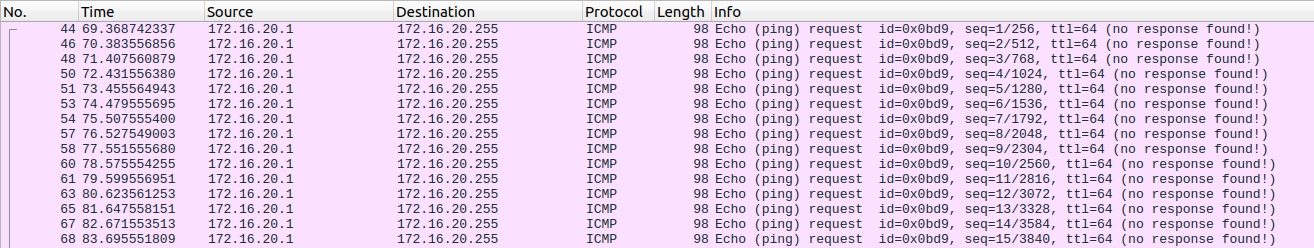
\includegraphics[width=\textwidth,height=\textheight,keepaspectratio]{imagens/exp2_tux23_broadcast.png}
\caption{Excerto de logs de ping em broadcast no tux23 na experiência 2}
\label{fig:exp2_tux23_broadcast}
\end{figure}

\begin{figure}[h!]
\centering
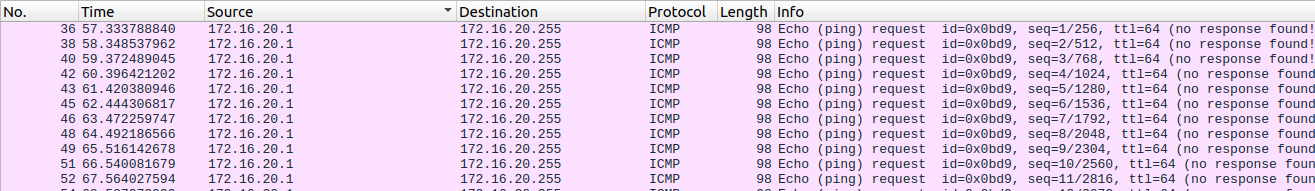
\includegraphics[width=\textwidth,height=\textheight,keepaspectratio]{imagens/exp2_tux24_broadcast.png}
\caption{Excerto de logs no tux24 durante ping em broadcast no tux23 na experiência 2}
\label{fig:exp2_tux24_broadcast}
\end{figure}

\begin{figure}[h!]
\centering
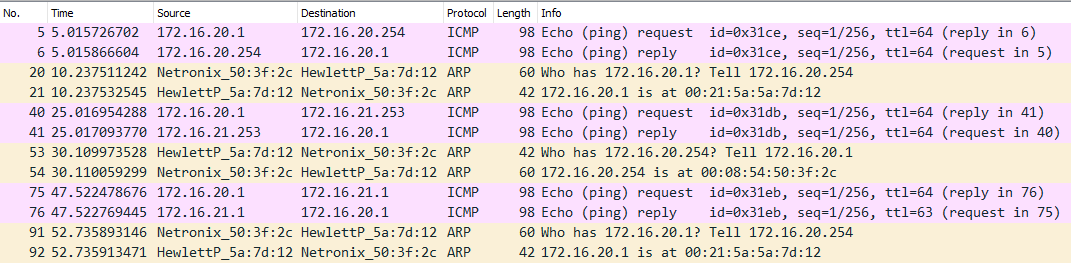
\includegraphics[scale=0.4]{imagens/exp3_tux3_logs.png}
\caption{Excerto de logs captados no tux23 na experiência 3}
\label{fig:exp3_tux3_logs}
\end{figure}

\begin{figure}[h!]
\centering
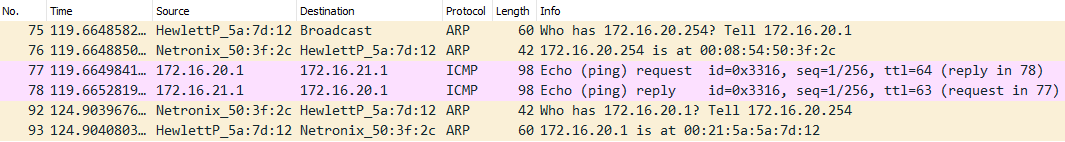
\includegraphics[scale=0.4]{imagens/exp3_tux4_eth0_logs.png}
\caption{Excerto de logs captados no tux24 eth0 na experiência 3}
\label{fig:exp3_tux4_eth0_logs}
\end{figure}

\begin{figure}[h!]
\centering
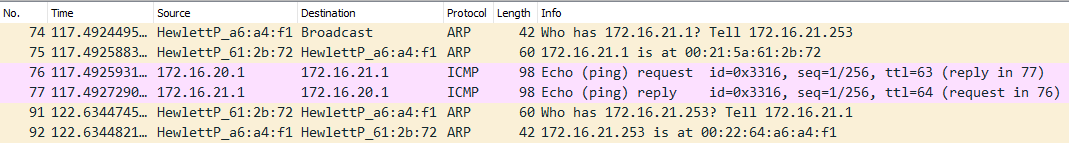
\includegraphics[scale=0.4]{imagens/exp3_tux4_eth1_logs.png}
\caption{Excerto de logs captados no tux24 eth1 na experiência 3}
\label{fig:exp3_tux4_eth1_logs}
\end{figure}

\begin{figure}[h!]
\centering
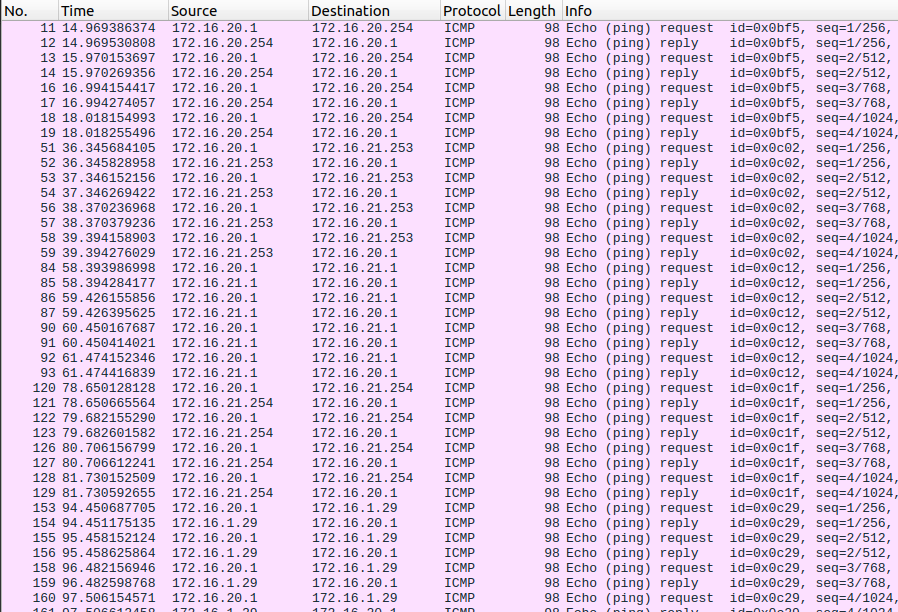
\includegraphics[scale=0.4]{imagens/exp4_tux23_ping_everything.png}
\caption{Excerto de logs no teste de conectividade do tux23 a todos os outros IP's na experiência 4}
\label{fig:exp4_tux23_ping_evertything}
\end{figure}

\begin{figure}[h!]
\centering
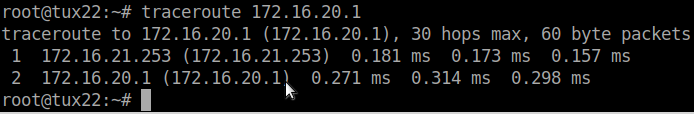
\includegraphics[scale=0.4]{imagens/exp4_traceroute_after_add_route.png}
\caption{traceroute após adicionar rota no tux22 até á interface eth0 do tux23 na experiência 4}
\label{fig:exp4_traceroute_after_add_route}
\end{figure}

\begin{figure}[h!]
\centering
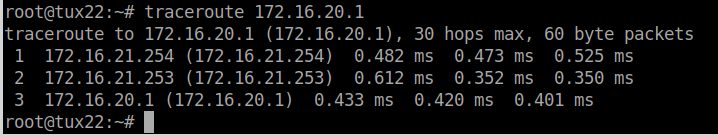
\includegraphics[scale=0.4]{imagens/exp4_traceroute_after_remove_route.png}
\caption{traceroute após remover rota no tux22 até á interface eth0 do tux23 na experiência 4}
\label{fig:exp4_traceroute_after_remove_route}
\end{figure}

\begin{figure}[h!]
\centering
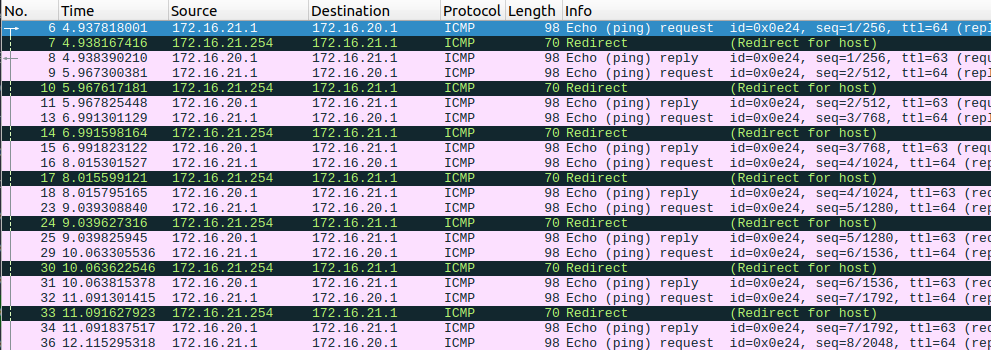
\includegraphics[scale=0.4]{imagens/exp4_tux22_ping_tux23_with_redirect.png}
\caption{Excerto de logs após remover rota no tux22 ao fazer ping do tux23 na experiência 4}
\label{fig:exp4_tux22_ping_tux23_with_redirect}
\end{figure}

\begin{figure}[h!]
\centering
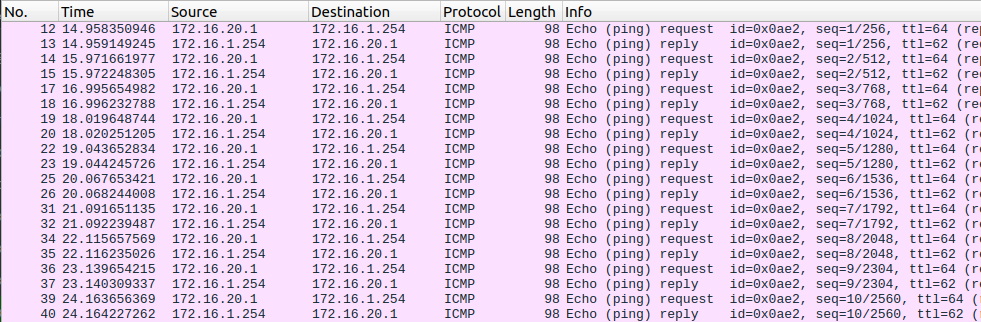
\includegraphics[scale=0.4]{imagens/exp4_tux23_ping_lab_router.png}
\caption{Excerto de logs captados no tux23 ao fazer ping do router do laboratório na experiência 4}
\label{fig:exp4_tux23_ping_lab_router}
\end{figure}

\begin{figure}[h!]
\centering
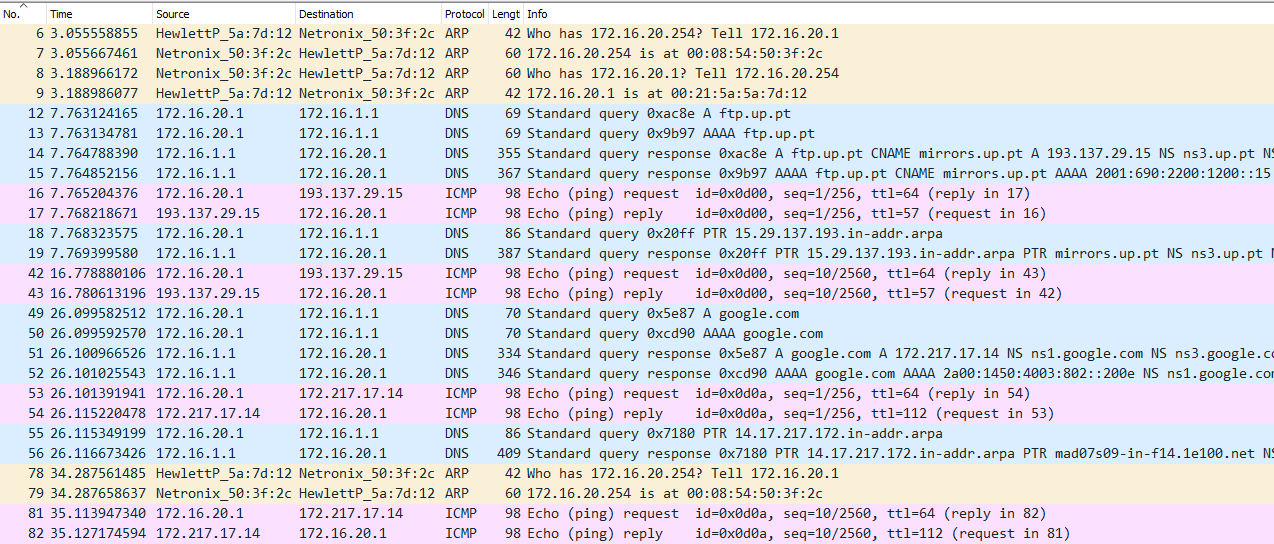
\includegraphics[scale=0.35]{imagens/exp5_logs.png}
\caption{Excerto de logs captados no tux23 eth0 na experiência 5}
\label{fig:exp5_logs}
\end{figure}

\begin{figure}[h!]
\centering
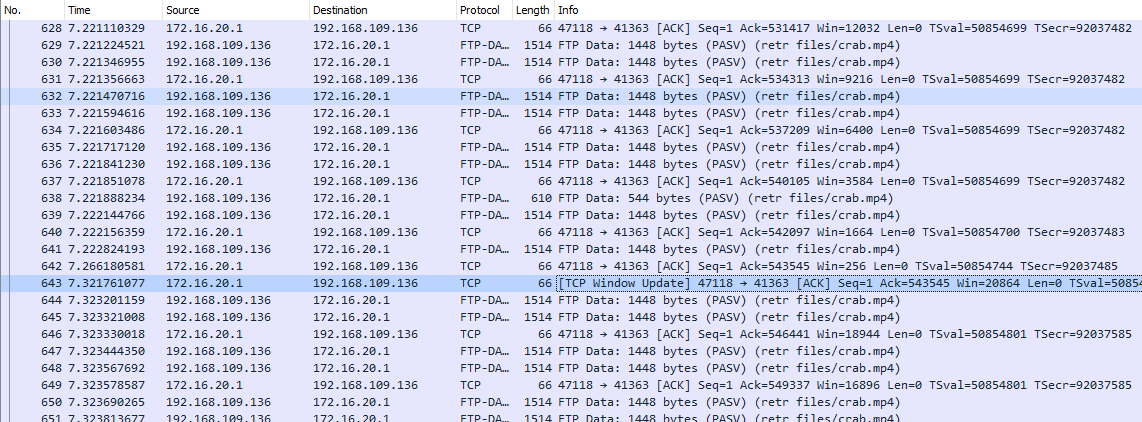
\includegraphics[scale=0.35]{imagens/exp6_logs_ACK_window_update.PNG}
\caption{Excerto de logs captados durante o download de um ficheiro na experiência 6}
\label{fig:exp6_logs_ACK_window_update}
\end{figure}

\begin{figure}[h!]
\centering
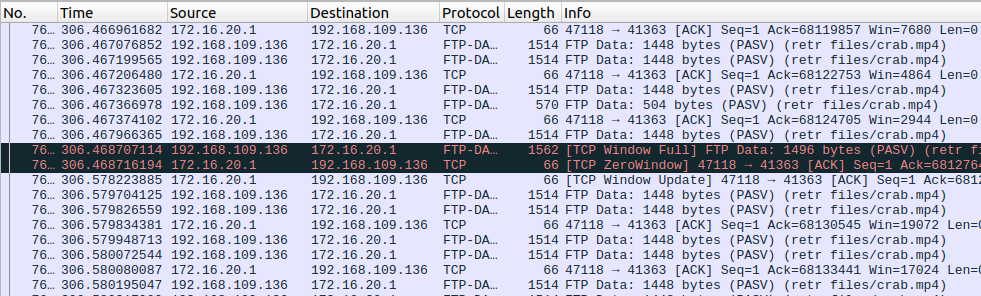
\includegraphics[scale=0.35]{imagens/exp6_window_full.png}
\caption{Excerto de logs captados durante o download de um ficheiro na experiência 6}
\label{fig:exp6_window_full}
\end{figure}

\begin{figure}[h!]
\centering
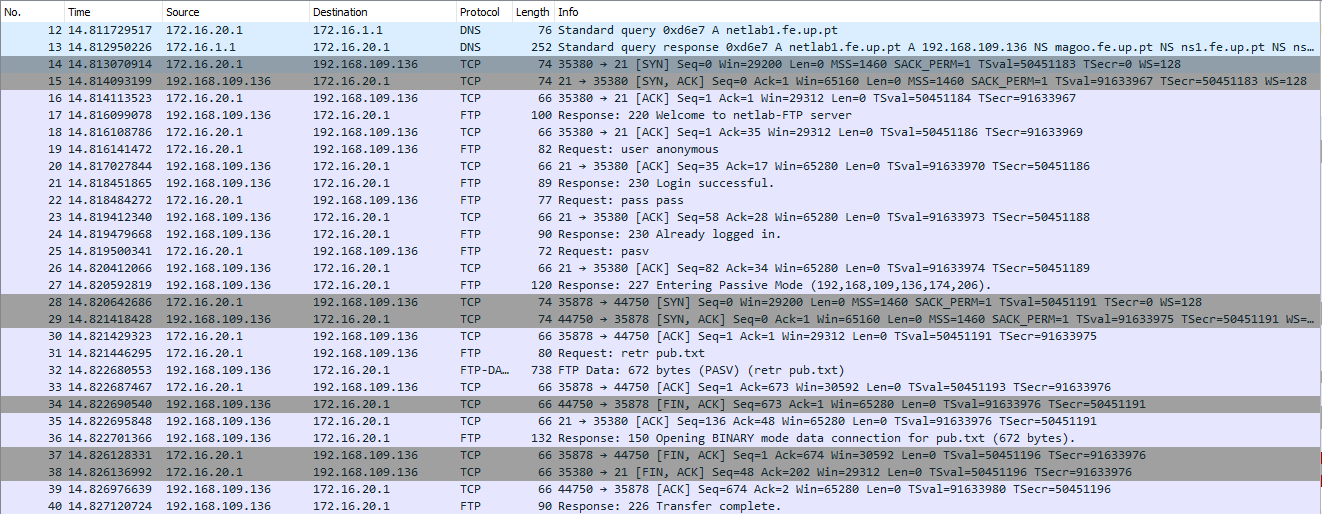
\includegraphics[scale=0.35]{imagens/exp6_download_steps.PNG}
\caption{Excerto de logs captados durante o download do ficheiro 'pub.txt' na experiência 6}
\label{fig:exp6_download_steps}
\end{figure}